\documentclass[11pt,a4paper]{article}
\usepackage[margin=1in]{geometry}
\usepackage{amsmath,amssymb,booktabs,tabularx,graphicx,hyperref}
\usepackage{tikz}
\hypersetup{colorlinks=true,urlcolor=blue,citecolor=blue}
\title{ZKP-Authorized Homomorphic Matching and Auditable Record Revocation for Organ Donation}
\author{Chirag Parmar\\M250738CS\\Department of Computer Science and Engineering\\National Institute of Technology Calicut\\Guided by Dr. Abidha V.P. and Dr. Bijoy Das}
\date{Major Project, Phase II --- revised October 2026}
\begin{document}
\maketitle
\begin{abstract}
This work implements a synthetic organ-donation research prototype combining institution-approved role membership, browser-generated zero-knowledge proofs, BFV homomorphic matching, encrypted IPFS storage and auditable local record revocation. Groth16 proofs bind membership to an intended wallet, chain, authorization contract and membership-root version. The backend is explicitly trusted for input encryption and permitted-result decryption; the system does not implement function-specific functional-encryption keys. Only opaque record identifiers, encrypted-content anchors and lifecycle metadata are registered on a local development blockchain. A fixed synthetic policy separates ABO eligibility from experimental feature/urgency ranking. A durable worker recovers missed revocation events and retries local cleanup. The evaluation separates cryptographic correctness, authorization enforcement, failure recovery and performance. Results establish prototype behavior under the stated assumptions, not clinical validity, anonymity, universal erasure or legal compliance.
\end{abstract}

\section{Problem and research questions}
The engineering problem is to control which approved stakeholders may register records, request an encrypted calculation and retire service access while preserving an auditable lifecycle. Blockchain auditability does not itself provide data confidentiality. Encryption during evaluation does not hide plaintext from a service that receives inputs and owns the decryption key. Zero-knowledge membership also requires an independently trustworthy enrollment process.

The research questions are: (RQ1) does approved membership enforce the specified role policy? (RQ2) what overhead does ZKP authorization introduce relative to wallet-based RBAC? (RQ3) do encrypted calculations agree with the independently specified plaintext policy? (RQ4) do encrypted records and revocation jobs recover after process restarts or listener downtime?

The contributions are a concrete protocol integration, an implementation with explicit trust boundaries, adversarial and recovery tests, and reproducible local measurements. No claim of a new FE scheme, new Merkle-tree algorithm or first-ever integration is made.

\section{Related work and positioning}
Hawashin et al. develop private-Ethereum smart contracts for organ-donation and transplantation management, including actor registration and lifecycle provenance~\cite{hawashin}. Their workflow motivates the distinction between an auditable lifecycle and confidential matching. This revision demonstrates selected registration, matching and retirement operations rather than a complete transplant-management system.

Vanin et al. investigate homomorphic encryption with blockchain and distributed off-chain storage for personal health records~\cite{vanin}. Their work establishes that encrypted healthcare computation and storage integration precede this prototype; the present evaluation concentrates on role enrollment, constrained output release and recovery behavior.

Egala, Pradhan and Gupta describe Block-Privacy using blockchain, IPFS, zero-knowledge protocols and functional encryption for IoMT~\cite{egala}. The publisher records first-online publication in October 2023 and a 2024 proceedings citation. Unlike an FE design, this implementation uses a trusted BFV secret-key holder. Claims about unexamined implementation details of prior work are deliberately omitted.

The earlier draft's Samsukha reference and other entries without verified primary-source metadata are tracked separately in \texttt{bibliography-verification.md}; unverified feature comparisons are not used to establish novelty. FE means function-dependent decryption capability~\cite{fe}; polynomial evaluation with BFV and an access-controlled server is not, by itself, FE.

\section{System and threat model}
\subsection{Actors and trusted components}
The institution administrator approves role-bound public membership leaves and may remove credentials. The participant browser creates and stores credential secrets and generates proofs in a worker. The trusted service sees submitted synthetic clinical attributes during encryption, owns the BFV decryption key and unwraps records for evaluation. SQLite holds public membership data, encrypted keys, canonical record mappings and durable jobs. Kubo stores AES-wrapped BFV bundles. Smart contracts record authorization and lifecycle metadata.

The blockchain operator, administrator, service operator, browser application origin and local setup contributor are trusted in this deployment. A compromised service can decrypt records available to it. A malicious application origin can steal browser credentials. Public development wallet keys are used only on isolated local chains. This is not a secure multi-hospital deployment.

\begin{figure}[ht]\centering
% Shared by the paper and presentation. Dashed boxes are trust domains.
\resizebox{\linewidth}{!}{%
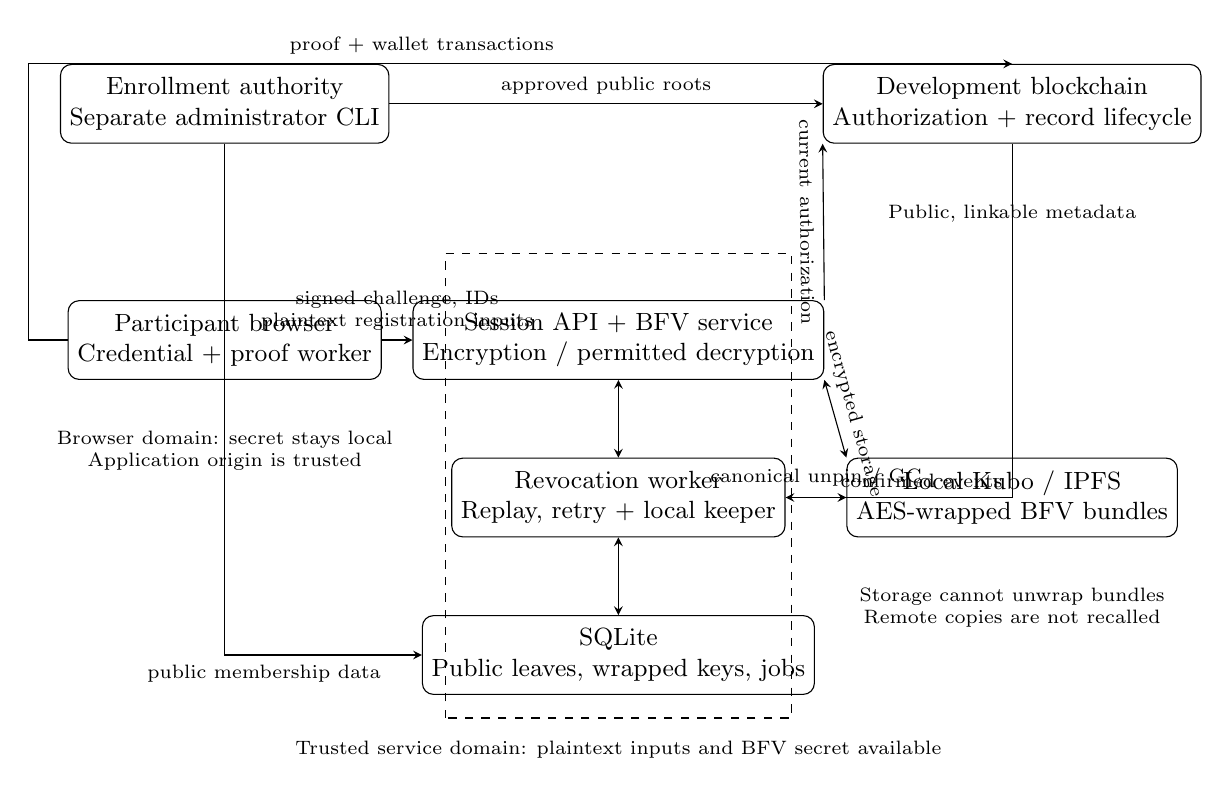
\begin{tikzpicture}[>=stealth,box/.style={draw,rounded corners,align=center,minimum width=3.3cm,minimum height=1cm,font=\small},every edge/.style={draw,->},every edge quotes/.style={font=\scriptsize}]
\node[box] (admin) at (-5,3) {Enrollment authority\\Separate administrator CLI};
\node[box] (browser) at (-5,0) {Participant browser\\Credential + proof worker};
\node[box] (chain) at (5,3) {Development blockchain\\Authorization + record lifecycle};
\node[box] (api) at (0,0) {Session API + BFV service\\Encryption / permitted decryption};
\node[box] (worker) at (0,-2) {Revocation worker\\Replay, retry + local keeper};
\node[box] (db) at (0,-4) {SQLite\\Public leaves, wrapped keys, jobs};
\node[box] (ipfs) at (5,-2) {Local Kubo / IPFS\\AES-wrapped BFV bundles};
\draw[dashed] (-2.2,-4.8) rectangle (2.2,1.1);
\node[font=\scriptsize,align=center] at (0,-5.2) {Trusted service domain: plaintext inputs and BFV secret available};
\draw[->] (admin) -- node[above,font=\scriptsize] {approved public roots} (chain);
\draw[->] (browser) -- node[above,font=\scriptsize,align=center] {signed challenge, IDs\\plaintext registration inputs} (api);
\draw[->] (browser.west) -- ++(-.5,0) |- node[pos=.7,above,font=\scriptsize] {proof + wallet transactions} (chain.north);
\draw[->] (api.north east) -- node[below,font=\scriptsize,sloped] {current authorization} (chain.south west);
\draw[->] (chain.south) |- node[pos=.7,above,font=\scriptsize] {confirmed events} (worker.east);
\draw[<->] (api) -- (worker);
\draw[<->] (worker) -- (db);
\draw[<->] (api.south east) -- node[above,font=\scriptsize,sloped] {encrypted storage} (ipfs.north west);
\draw[->] (worker) -- node[above,font=\scriptsize] {canonical unpin / GC} (ipfs);
\draw[->] (admin.south) |- node[pos=.6,below,font=\scriptsize] {public membership data} (db.west);
\node[font=\scriptsize,align=center] at (-5,-1.4) {Browser domain: secret stays local\\Application origin is trusted};
\node[font=\scriptsize,align=center] at (5,1.6) {Public, linkable metadata};
\node[font=\scriptsize,align=center] at (5,-3.4) {Storage cannot unwrap bundles\\Remote copies are not recalled};
\end{tikzpicture}%
}

\caption{Protocol components and trust boundaries. Administrative signing keys stay outside the API process. The trusted service sees registration inputs and owns decryption capability; ciphertext storage and public blockchain metadata have different visibility.}
\end{figure}

\subsection{Adversary and leakage}
Tests cover unregistered users, role misuse, expired/revoked authorization, stolen proof submission, arbitrary-ciphertext decryption attempts, inconsistent records and service/storage failure. Observers still see wallet addresses, roles, timing, opaque record identifiers, entity types and lifecycle activity. Membership leaves are public commitments to high-entropy secrets. Scores reveal information about input relationships; repeated chosen-record queries can reveal more. Output restrictions and quotas do not establish FE, differential privacy or resistance to all inference attacks.

\section{Protocol}
\subsection{Enrollment and browser proof}
A browser samples a 248-bit random secret $s$. A role leaf is $L=H(s,r)$, where $H$ is circomlib-compatible Poseidon with two inputs and $r\in\{0,\ldots,5\}$. The administrator approves $L$ in a persistent depth-20 tree. Authentication never changes the root. A root update increments its version and invalidates earlier role sessions.

Private circuit inputs are $s$, fresh salt $\rho$ and the Merkle path. Path selectors are constrained to $b(b-1)=0$. Public inputs are the root, role, nullifier, recipient wallet, chain identifier, issuer contract and root version. The nullifier is
\[
n=H(s,H(\rho,H(\mathrm{wallet},H(\mathrm{chain},H(\mathrm{issuer},\mathrm{version}))))).
\]
The contract verifies the proof, current root/version, domain and intended sender, and rejects a used nullifier. It creates a four-hour authorization session. This is an authorization record, not a cryptographic functional key. A wallet-signed, five-minute single-use challenge then establishes an API bearer session whose expiry cannot exceed the on-chain expiry. Every protected operation rechecks current authorization.

The worker hashes fetched WASM and proving-key artifacts before use. Setup includes a secret phase-two contribution and transcript verification against the compiled R1CS and prepared ptau. The inherited local phase-one transcript and single-contributor phase-two trust remain limitations; independent multiparty setup is not claimed~\cite{groth}.

\subsection{Roles}
\begin{center}
\begin{tabular}{lcccc}
\toprule Role & Donor registration & Recipient registration & Matching & Revocation\\\midrule
Doctor & Yes & Yes & Yes & No\\
Coordinator & Yes & Yes & Yes & No\\
Procurement & Yes & No & Yes & No\\
Matching & No & No & Yes & No\\
Transporter & No & No & No & No\\
Surgeon & No & No & Yes & Yes\\\bottomrule
\end{tabular}
\end{center}
Transport and transplant confirmation are not implemented capabilities in this revision. Administrative retention scheduling is separate from these stakeholder permissions.

\subsection{Record storage and key custody}
Each record contains two encrypted ABO flags, six encrypted binary synthetic tissue features and encrypted urgency: nine BFV ciphertexts. These are toy features, not clinical HLA typing. BFV uses polynomial degree 4096, SEAL's tc128 default coefficient modulus and a 20-bit batching plaintext modulus. The implementation checks result bounds and a positive noise budget~\cite{seal}.

The ciphertext bundle is wrapped with a fresh record-specific AES-256-GCM key using the opaque record ID as authenticated context. The BFV secret and record keys are encrypted at rest under an operator-provided wrapping secret. Missing or incorrect keys cause failure; keys are not silently replaced. The canonical CID remains off-chain; the chain records its hash alongside the opaque record ID, entity type, registrant and activity metadata. Plaintext ABO, urgency and feature values are absent from transaction inputs, contract storage and events.

The authorized API prepares the bundle, the participant wallet registers its anchor, and confirmation validates the canonical owner/type/anchor. Matching accepts only record IDs and a fixed function. It does not accept arbitrary ciphertexts, weights or requested decryptions. Batch jobs cache encrypted bundles within the job, avoiding repeated storage retrieval for the same record; canonical activity and authorization checks remain in place. API result release rechecks authorization and record activity.

\section{Synthetic matching specification}
The ordinary synthetic ABO policy permits O to any ABO group, A to A/AB, B to B/AB and AB to AB. Rh and incompatible-transplant exceptions are outside scope. With encrypted A/B flags, incompatibility is
\[
I=A_D(1-A_R)+B_D(1-B_R).
\]
Only $I=0$ is eligible. Ineligible pairs receive no ranking score.

For six binary synthetic features and recipient urgency $u\in\{0,1,2\}$,
\[
m=\sum_{k=1}^{6}(d_k-r_k)^2,\qquad
N=4200-700m+900u,\qquad
S=\operatorname{round}(N/6).
\]
BFV evaluates $I$ and $N$. The trusted service releases eligibility and, for eligible pairs, $S$. Bounds are $0\le m\le6$, $0\le N\le6000$ and $0\le S\le1000$. All coefficients are experimental. The UI labels $S$ as synthetic ranking points, never a clinical probability or compatibility percentage. Ties use donor then recipient ID. Ranking neither reserves organs nor computes an optimal assignment.

\section{Auditable local revocation}
For either record type, the surgeon requests and executes deactivation by opaque ID. The contract does not accept an arbitrary CID. Canonical chain deactivation blocks evaluation independently of cleanup progress. A durable worker scans confirmed logs, checkpoints block/hash metadata, deletes the service-held record key and retries canonical local unpin/GC work. Cleanup errors remain visible. A bounded scheduling cursor inspects at most 50 entries per call, including not-yet-due entries.

State reporting distinguishes requested, deactivated, cleanup pending, completed locally and failed. A detected change to processed chain history halts cleanup for audit because deletion is irreversible. Event catch-up handles downtime; it does not make already deleted keys recoverable after a deep reorganization.

Local unpinning cannot erase remote replicas~\cite{ipfs}. Deleting a live key does not erase backups, copied keys or prior outputs. Accordingly, the implementation demonstrates local retention/access revocation under operator assumptions. It does not establish GDPR compliance. Any deployment would require a lawful basis, applicable retention policy and assessment of erasure exceptions; data minimisation is Article 5(1)(c)~\cite{gdpr}.

\section{Evaluation methodology and evidence}
Tests distinguish real Groth16 contract verification, mocked HTTP/recovery fault injection and a live browser/API/Kubo/chain demonstration. The live script uses an EIP-1193 development-wallet adapter, not the MetaMask extension UI. It checks enrollment rejection, browser proving, encrypted storage, matching, restart recovery, both record-type revocations and absence of credential secrets in API request bodies.

The enabled full validation run completed 28 passing tests with zero skipped tests; its live demonstration passed 11 checks, including fail-closed startup when key metadata is missing against existing on-chain records. The default test command explicitly skips live infrastructure unless enabled. The repository's \texttt{claim-evidence-v2.md} maps these claims to implementation files and recorded evidence.

Repeated enrollment, proving, encryption, evaluation, release, storage, authorization-receipt, revocation and HTTP-job timing experiments use ten warmups and thirty measured repetitions; raw samples, median, p95 and variability are retained. Initial authorization issuance gas is recorded separately from the warmed samples that update an existing session slot. The same authenticated HTTP job interface runs 1-by-1, 5-by-5 and 10-by-10 workloads for plaintext wallet RBAC, BFV wallet RBAC and BFV ZKP authorization. Plaintext baseline data stays in memory while BFV retrieves AES-wrapped records from real local Kubo, so the measured difference includes storage/protection costs rather than isolating cryptography alone. Benchmark-only quotas are raised in the isolated harness; application quotas remain enforced. Node proving timing includes witness-input/path construction; browser execution is separate acceptance evidence.

Source/artifact hashes, parent commit, dirty-working-tree designation, hardware and versions identify the evaluated revision. Request and execution gas are reported separately. Revocation alternates donor and recipient records and measures request, execution and direct cleanup separately; cleanup timing excludes worker discovery and retry delay. Initial dataset-registration gas has twenty samples. The local EVM does not measure consortium consensus or public-network finality.

HTTP-job timings include submission and polling every 100 milliseconds until results are available, using fresh HTTP connections. Any bounded retry of an idempotent polling transport failure is recorded and remains inside the timed sample; POST requests are never replayed. This adds latency quantization and an observation overhead, particularly for the plaintext and one-pair cases. Empirical medians use the upper middle order statistic for the even-sized sample; p95 uses the nearest-rank order statistic.

Workload comparisons use an already established API session in each baseline. A new ZKP is not generated for each pair or job; proof generation and on-chain authorization are measured separately and their cost is amortized over the session. Consequently, job-latency differences alone do not measure the full login cost of ZKP authorization.

Baselines run sequentially in a fixed order on one machine. Host scheduling, thermal variation and order effects are not experimentally controlled. The descriptive statistics characterize this run; small differences between the two BFV baselines are not evidence of a causal speedup or slowdown without independent counterbalanced repetitions.

Scaling workloads use O donors with features $(1,0,1,0,1,0)$ and A recipients with features $(1,1,1,0,0,0)$, cycling urgency through $0,1,2$. Thus every workload pair is eligible with two feature mismatches; record identifiers are freshly randomized. These fixtures exercise the score-release path rather than representing a clinical population. All ABO combinations and randomized feature values are assessed separately in correctness tests.

\IfFileExists{results-v2.tex}{\paragraph{Measured local results.} Ten warmups and thirty measured samples were used for every repeated timing metric below. The table reports milliseconds; Node proving includes path construction and is not a browser latency measurement. Local receipt times exclude real-network consensus; direct cleanup excludes worker discovery and retry delay.
\begin{center}\begin{tabular}{lrrr}\toprule Metric & Median (ms) & p95 (ms) & SD (ms)\\\midrule
Approved-root enrollment & 38.58 & 45.93 & 4.69\\
Membership witness construction & 47.82 & 50.29 & 1.01\\
Node Groth16 proving & 2922.25 & 4318.04 & 1168.12\\
Local authorization receipt & 10.45 & 11.76 & 0.86\\
BFV record encryption & 115.16 & 131.60 & 8.89\\
BFV policy evaluation & 230.73 & 244.98 & 7.60\\
Permitted-result release & 10.47 & 16.85 & 2.76\\
Encrypted storage round trip & 42.03 & 107.35 & 20.37\\
Local revocation request receipt & 1.87 & 2.41 & 4.94\\
Local deactivation receipt & 1.66 & 2.07 & 0.23\\
Direct local cleanup & 22.62 & 31.28 & 5.13\\
\bottomrule\end{tabular}\end{center}
\paragraph{Verification gas.} Median real Groth16 verification plus authorization issuance: 310,463 gas (30 measured samples after ten warmups). Initial issuance, recorded separately: 367,339 gas; warmed samples reuse the same wallet session slot.
\paragraph{Workload interpretation.} The plaintext baseline uses memory-resident synthetic data, while BFV uses real encrypted Kubo records. Differences include storage and protection costs; they do not isolate proof cost. Jobs use an established session, with proving and authorization measured separately rather than repeated per job. Job timings include 100-ms result polling, which affects small-workload latency. Raw samples and source/artifact identifiers accompany the evaluation.
\begin{center}\begin{tabular}{llrrr}\toprule Baseline & Matrix & Median (ms) & p95 (ms) & SD (ms)\\\midrule
Plaintext wallet RBAC & 1x1 & 134.88 & 146.71 & 6.54\\
Plaintext wallet RBAC & 5x5 & 291.90 & 336.71 & 47.04\\
Plaintext wallet RBAC & 10x10 & 862.31 & 1080.33 & 72.85\\
BFV wallet RBAC & 1x1 & 384.68 & 599.39 & 85.15\\
BFV wallet RBAC & 5x5 & 7203.02 & 7486.88 & 173.74\\
BFV wallet RBAC & 10x10 & 11946.91 & 17289.18 & 1464.74\\
BFV ZKP authorization & 1x1 & 164.48 & 198.90 & 11.34\\
BFV ZKP authorization & 5x5 & 3292.05 & 3423.10 & 77.39\\
BFV ZKP authorization & 10x10 & 12116.84 & 12406.25 & 148.14\\
\bottomrule\end{tabular}\end{center}
}{\paragraph{Results status.}Final numerical results remain provisional. Run the revised tests, live demonstration and benchmark suite; do not reuse historical prototype measurements.}
\IfFileExists{evaluation-v2/workload-latency.pdf}{\begin{figure}[ht]\centering
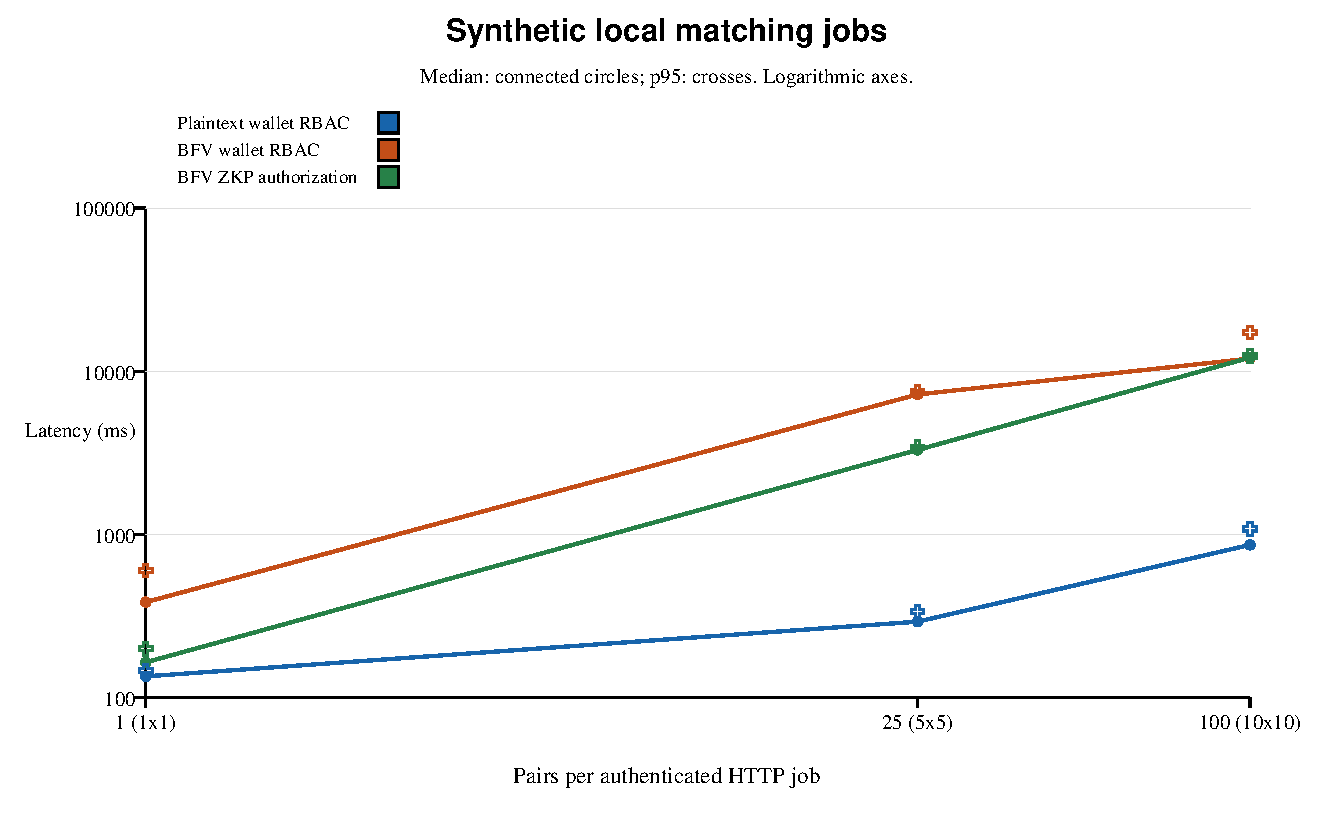
\includegraphics[width=\linewidth]{evaluation-v2/workload-latency.pdf}
\caption{Authenticated synthetic local matching jobs: median latency as lines and p95 as crosses. Baseline differences include storage/protection costs; this is not a clinical-benefit or consortium-throughput measurement.}
\end{figure}}{}

\section{Limitations and future work}
The toy binary-feature model and experimental weights are unvalidated for clinical decisions. The backend sees submitted inputs and can decrypt stored BFV records; general service compromise remains outside the confidentiality guarantee. Metadata is linkable. SQLite and a local wrapping secret are prototype key custody, not production HSM isolation. Revocation cannot recall external copies, historical outputs or backups. Browser wallet simulation does not substitute for manual extension testing. A local verified setup transcript does not replace independent multiparty contributions. Production deployment also requires dependency remediation and operational review.

Future work includes clinically reviewed eligibility/allocation models, multi-institution governance, stronger key custody, formal leakage analysis and independently verified setup. Actual FE and post-quantum components would require separate constructions and evaluation; adding one primitive would not make the whole current stack post-quantum.

\section{Conclusion}
The revised prototype evaluates approved role authorization, fixed BFV matching, confidential off-chain records and recoverable local revocation under explicit trust assumptions. Its scientific claim is the behavior and cost of this implementation under a reproducible synthetic workload, not a new cryptographic scheme or a clinically deployable allocation system.
\bibliographystyle{plain}
\bibliography{references-v2}
\end{document}
